\section{Success and failure cases}
\label{sec:cases}

The experiments as presented in previous sections provide insight into the general performance of our RNN-\nobreak{}based algorithms. In this section we look at individual cases, in order to identify when exactly the algorithm fails, and when it succeeds. Only a few cases are presented here, which are chosen to represent common mistakes. We note that since this is only a selection, it does not cover all success and failure cases. Furthermore, since we are dealing with individual cases we only describe our observations based on these examples, without making hard conclusions of the performance overall.

In Figure \ref{fig:sf_mono_rnn_not_bls}, we see the RNN and Mono-BLS applied to a light curve from the LCSim-Mono data set. In this case, the RNN was able to detect the planet, while for Mono-BLS the SNR did not exceed the detection threshold. This is likely due to the fact that the box-fitting algorithm picked up more noise than the RNN. For Mono-BLS, it seems that each fluctuation in brightness triggers some response to a transit event, while the RNN is relatively robust against this noise. We expect this to be the reason that a better threshold could be set with the RNN, in terms of the tradeoff between precision and recall, compared to the Mono-BLS algorithm.

\begin{figure}
    \centering
    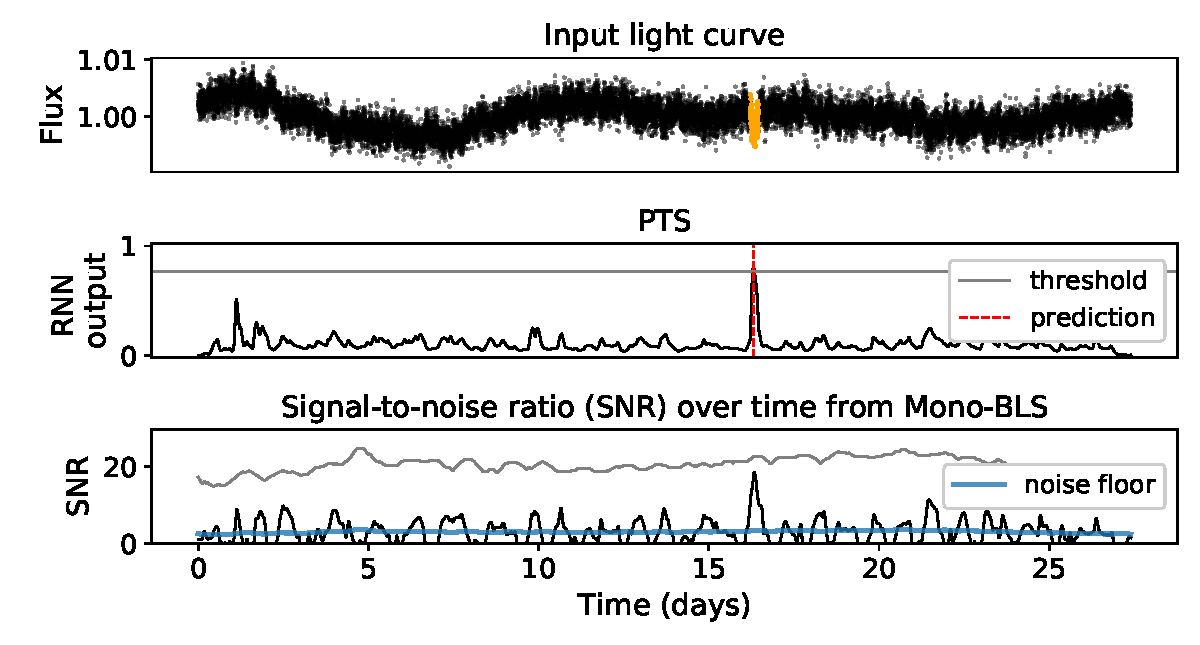
\includegraphics[width=0.65\linewidth]{Experiments/Figures/Cases/sf_mono_rnn_not_bls_3.pdf}
    \caption{An example of where the RNN succeeds and Mono-BLS fails in the task of monotransit retrieval. A detection threshold is set closest to a corresponding detection precision of 0.5 over the entire LCSim-Mono data set. The transit signal in the top figure is visualized in orange and a detection above the threshold is indicated with a dashed red line.}
    \label{fig:sf_mono_rnn_not_bls}
\end{figure}

When periodicity is involved, we found BLS to outperform our RNN-based algorithms in Section \ref{sec:singles}. Especially in the small period regime (e.g. see Figure \ref{fig:sf_single_bls_not_fold}), we found the RNN-based algorithms struggle with the fact that it relies on the detection of individual events, only after which the period of the signal is determined. BLS on the other hand, uses the periodicity to its advantage by folding the input light curve, effectively increasing the SNR of the signal. Still, in cases where the input light curve is very noisy, as shown in Figure \ref{fig:sf_single_fold_not_bls}, we found the RNN to be able to distinguish signals from the background, allowing PTS-Fold to detect the planet while BLS failed to do so. PTS-Fold and PTS-Peak are compared in Figure \ref{fig:sf_single_fold_not_peak}, where we see how the lack of strong peaks in the PTS can lead to PTS-Peak failing, while PTS-Fold still succeeds.

\begin{figure}
    \centering
    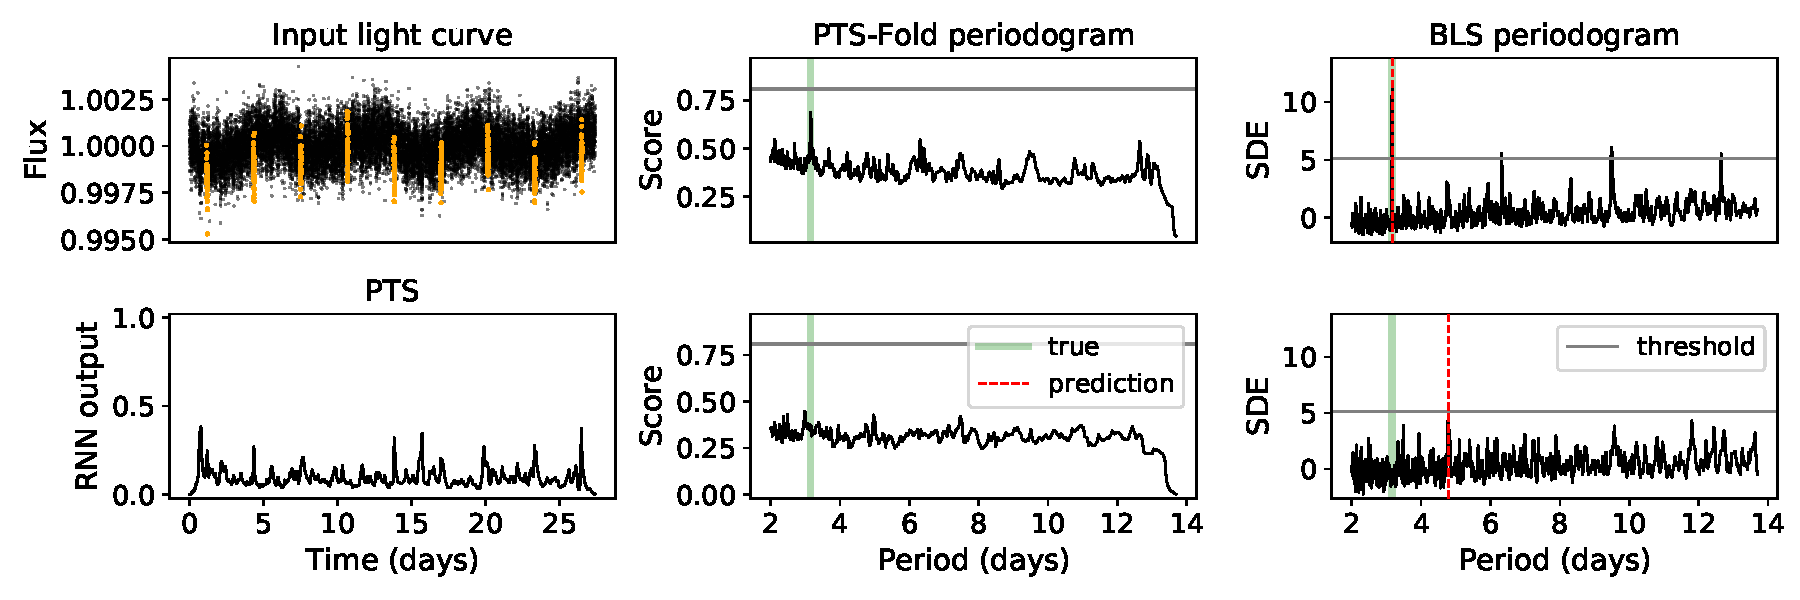
\includegraphics[width=\linewidth]{Experiments/Figures/Cases/sf_single_bls_not_fold_2.pdf}
    \caption{An example of where BLS succeeds and PTS-Fold fails in the task of retrieving repeating transit signals from a single planet. A detection threshold is set closest to a corresponding detection precision of 0.5 over the entire LCSim-Single data set. Transit signals are visualized in orange and a detection above the threshold is indicated by a dashed red line. Two steps of each method are visualized from top to bottom, where the top shows the initial periodogram, and the bottom shows the periodogram after the strongest signal has been removed.}
    \label{fig:sf_single_bls_not_fold}
\end{figure}

\begin{figure}
    \centering
    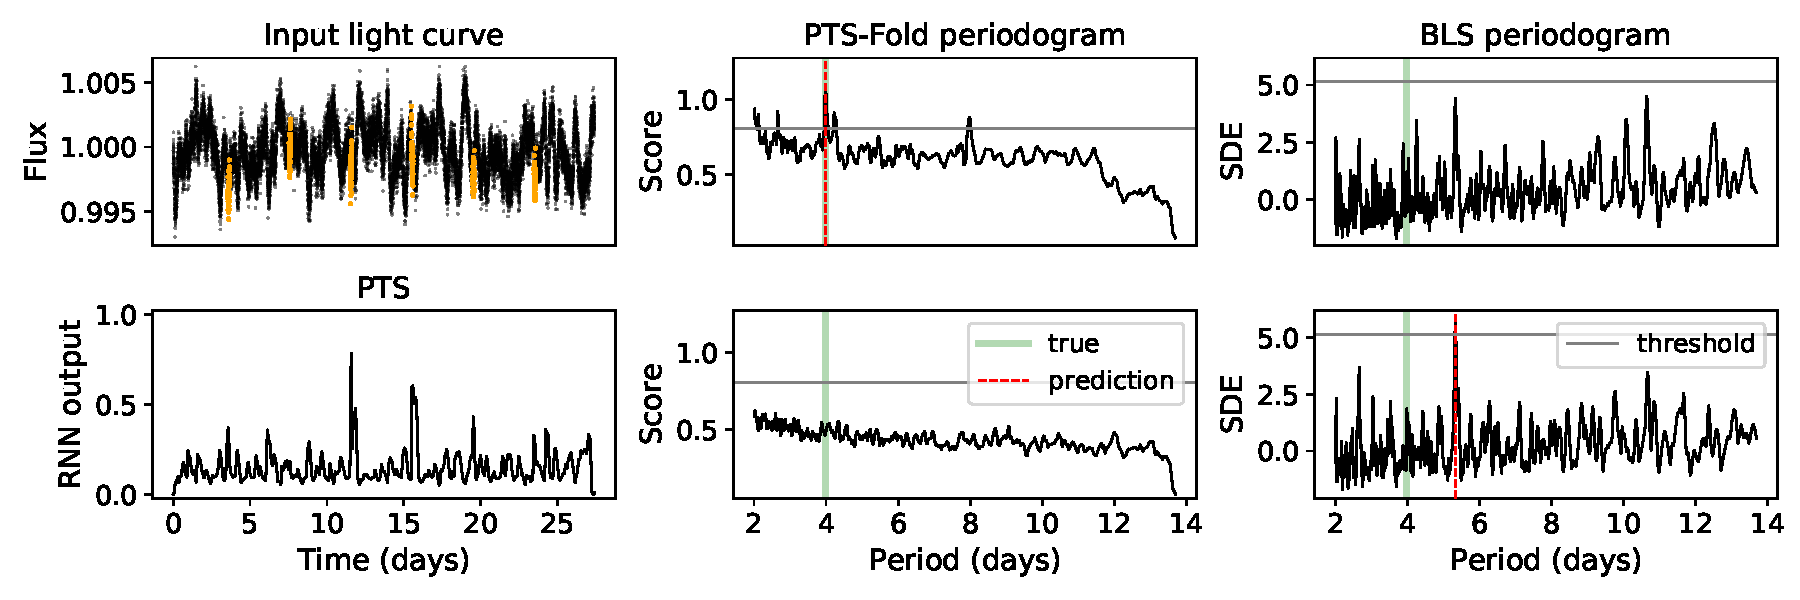
\includegraphics[width=\linewidth]{Experiments/Figures/Cases/sf_single_fold_not_bls_1.pdf}
    \caption{An example of where PTS-Fold succeeds and BLS fails in the task of retrieving repeating transit signals from a single planet. A detection threshold is set closest to a corresponding detection precision of 0.5 over the entire LCSim-Single data set.}
    \label{fig:sf_single_fold_not_bls}
\end{figure}

\begin{figure}
    \centering
    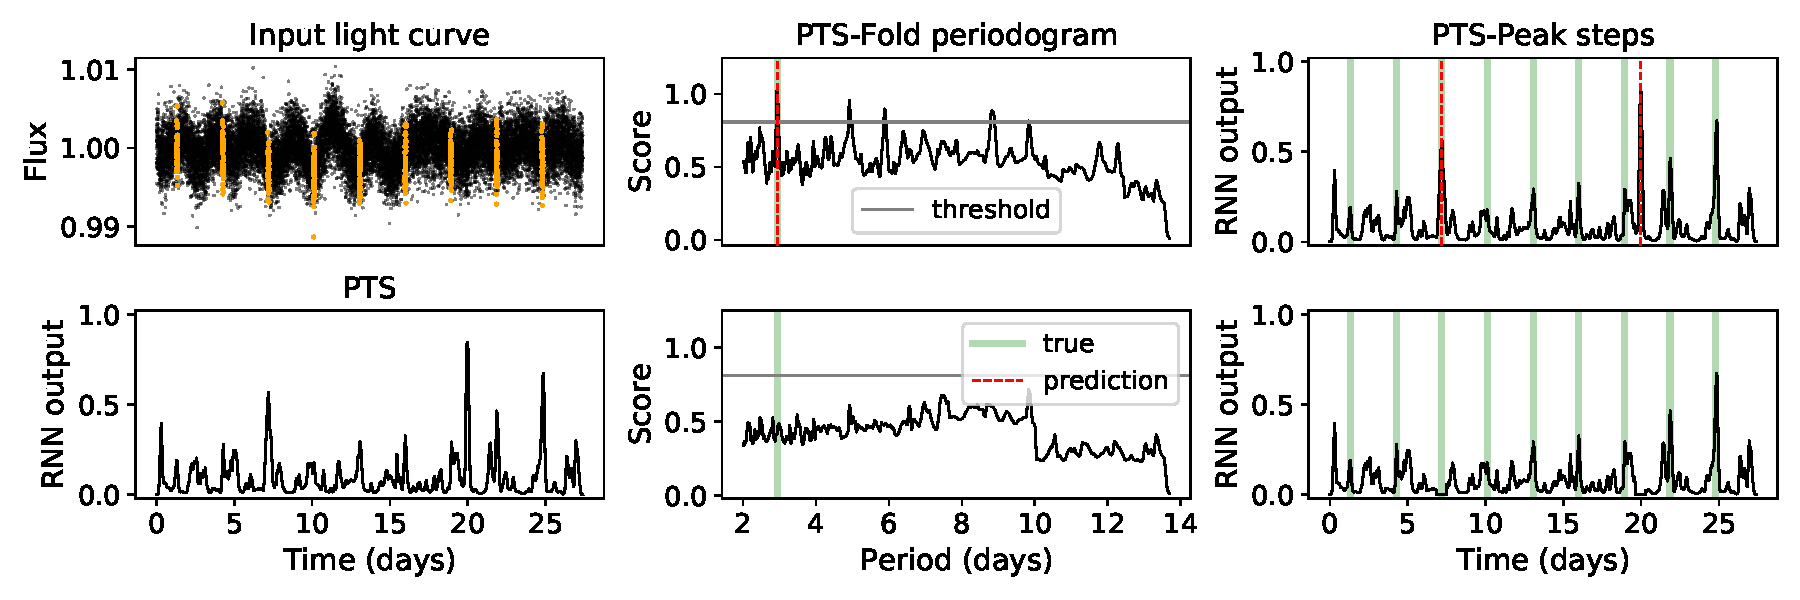
\includegraphics[width=\linewidth]{Experiments/Figures/Cases/sf_single_fold_not_peak_1.pdf}
    \caption{An example of where PTS-Fold succeeds and PTS-Peak fails in the task of retrieving repeating transit signals from a single planet. A detection threshold is set closest to a corresponding detection precision of 0.5 over the entire LCSim-Single data set. Two steps of both methods are shown from top to bottom. For PTS-Peak the top figure shows the original PTS, with green colors indicating the location of true transit signals, and red dashed lines indicating the predicted transit signals. The lower figure shows the PTS where the detected signal is removed.}
    \label{fig:sf_single_fold_not_peak}
\end{figure}
For Lilith light curves, shown in figures \ref{fig:sf_multi_viceversa} and \ref{fig:sf_multi_not_peak}, several things were observed. Firstly, the PTS seems to be less noisy compared to the PTS obtained with LCSim data. For this reason, the PTS-Fold periodogram is also cleaner.  Although this seems like a good thing, it also means that a transit signal is either detected, or not at all. This is likely the reason for the high precision at low recall of the RNN-based detection algorithms applied to Lilith data. We expect that a bit of noise in the PTS is beneficial to the algorithm, as it allows more planets to be detected at lower precision. 

\begin{figure}
    \centering
    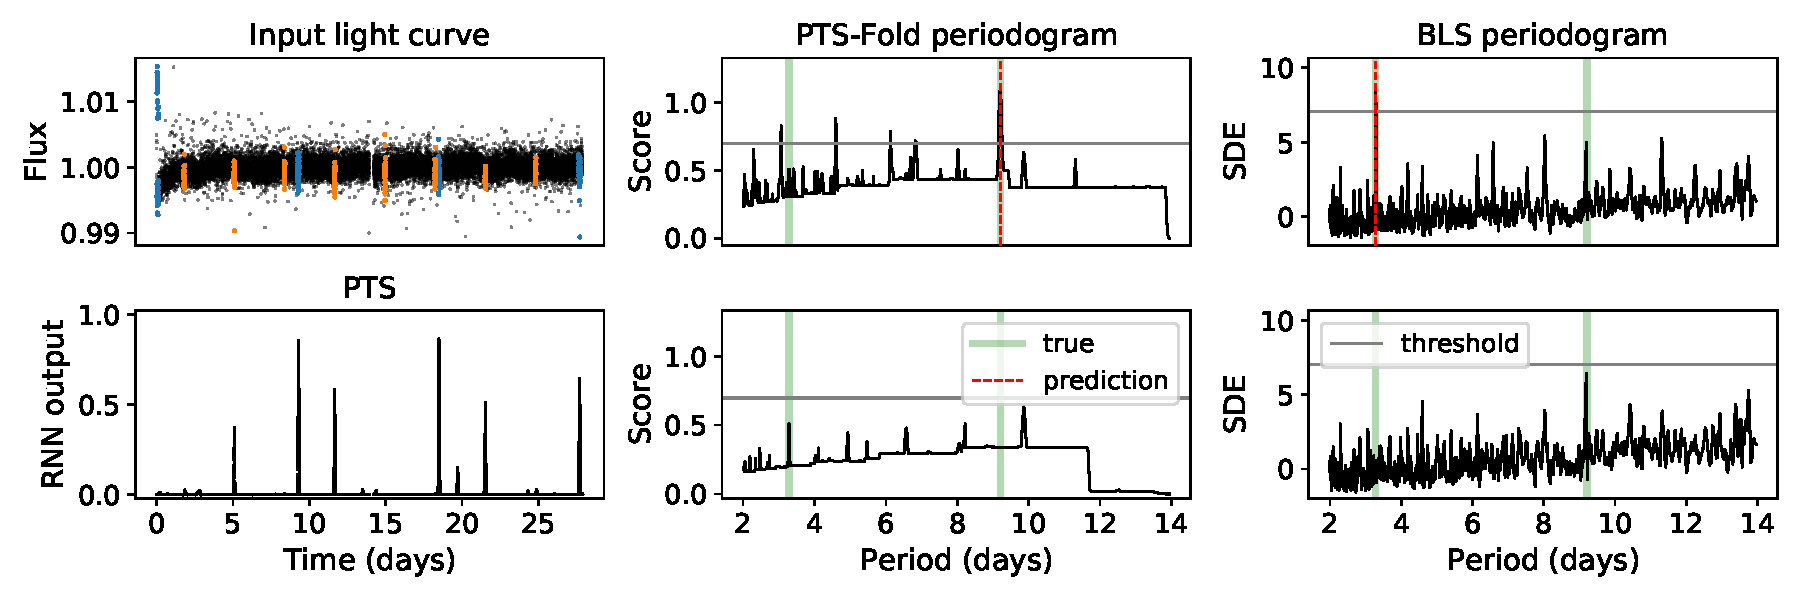
\includegraphics[width=\linewidth]{Experiments/Figures/Cases/sf_multi_vice.pdf}
    \caption{An example of where BLS and PTS-Fold both detect a planet that the other method was not able to detect. The input is a Lilith light curve with transit signals from two planets, indicated by blue and orange in the top left figure. A detection threshold is set closest to a corresponding detection precision of 0.5 over the entire Lilith-Multi data set.}
    \label{fig:sf_multi_viceversa}
\end{figure}

Secondly,  we found that our algorithms are prone to match the signals from two different planets together, which could lead to false detections. This phenomenon is made clear in Figure \ref{fig:sf_multi_not_peak}, where the wrong peaks in the PTS are combined by PTS-Peak to define a detection. This behaviour can be understood by the fact that peaks in the PTS carry little information about the shape of the detected signal in the light curve. Only the duration of a signal can be directly encoded in the PTS. For other features, we resort to the representations learned by the representation RNN from Section \ref{sec:representations}. Figure \ref{fig:sf_repr_3} shows that, even though the signals in the light curve are visually different, the peaks in the PTS are similar enough for PTS-Peak to match the wrong signals together. This could, however, be prevented if the signal representations are taken into account, which are separated in representation space. The representations are in this case two-dimensional, and the angle between two representations indicates how different they are. Figure \ref{fig:sf_repr_2} shows another example of this failure case, where the two signals are now more similar. The representations are therefore also closer to each other, but still can be separated in representation space.

\begin{figure}
    \centering
    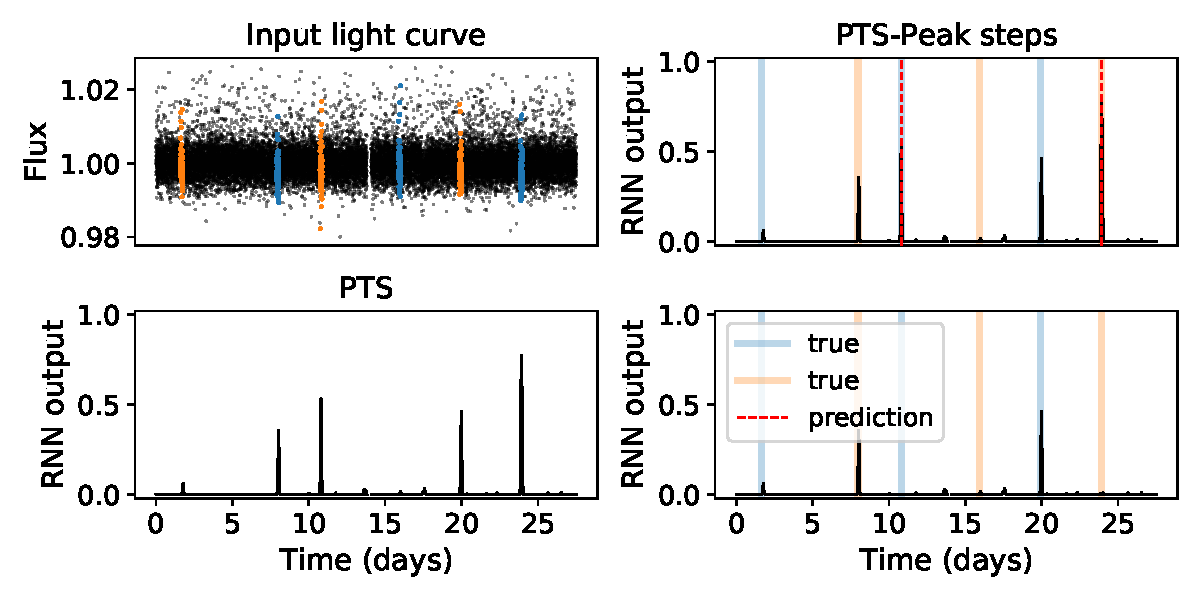
\includegraphics[width=0.6\linewidth]{Experiments/Figures/Cases/sf_multi_not_peak_2.pdf}
    \caption{An example of where PTS-Peak fails to match the peaks corresponding to the same signal for a given Lilith light curve. The colors indicate which transit signal belongs to which planet. The dashed line indicates the peaks that are extracted to define a detection, which in this case include peaks from two different planets.}
    \label{fig:sf_multi_not_peak}
\end{figure}

\begin{figure}
    \centering
    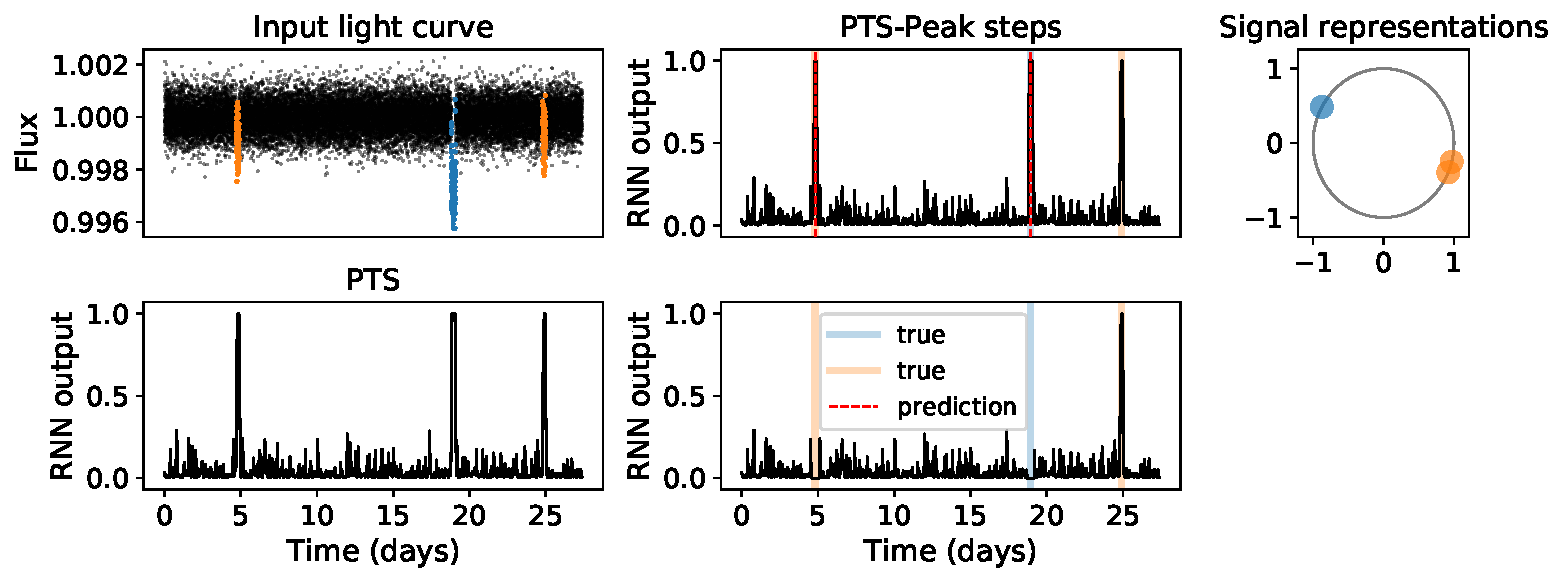
\includegraphics[width=0.85\linewidth]{Experiments/Figures/Cases/sf_multi_peak_repr_3.pdf}
    \caption{An example of how PTS-Peak may falsely match signals together from different planets, leading to incorrect detections. This problem could be prevented by using learned representations of transit signals, shown in the upper right. The dots represent the aggregated representations over all time steps withing a given peak in the PTS. The colors correspond to the colors used in the upper left figure. The light curve in this example consists exclusivey of white-noise.}
    \label{fig:sf_repr_3}
\end{figure}


\begin{figure}
    \centering
    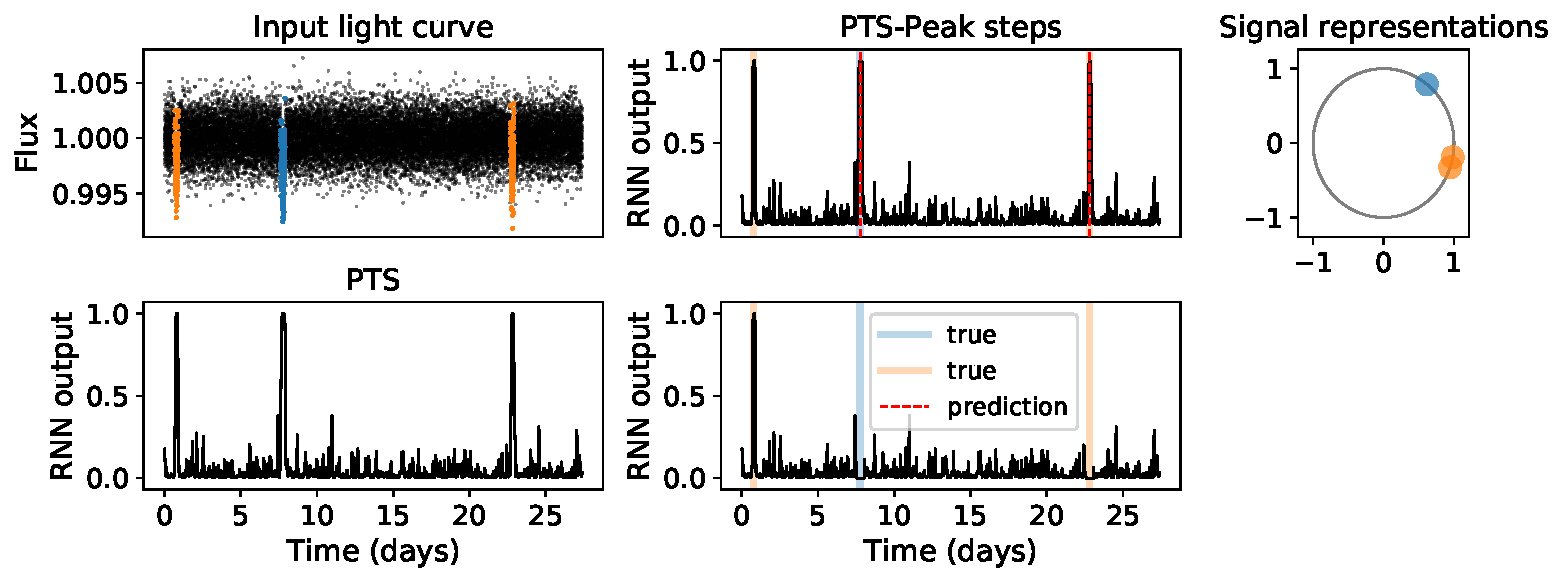
\includegraphics[width=0.85\linewidth]{Experiments/Figures/Cases/sf_multi_peak_repr_2.pdf}
    \caption{Another example of how the use of learned signal representations could have prevented PTS-Peak from matching the wrong peaks together in the PTS.}
    \label{fig:sf_repr_2}
\end{figure}
